% Adjust these for the path of the theme and its graphics, relative to this file
%\usepackage{beamerthemeFalmouthGamesAcademy}
\usepackage{../../beamerthemeFalmouthGamesAcademy}
\usepackage{multimedia}
\graphicspath{ {../../} }

% Default language for code listings
\lstset{language=C++,
        morekeywords={each,in,nullptr}
}

% For strikethrough effect
\usepackage[normalem]{ulem}
\usepackage{wasysym}

\usepackage{pdfpages}

% http://www.texample.net/tikz/examples/state-machine/
\usepackage{tikz}
\usetikzlibrary{positioning,shapes,shadows,arrows,automata}

\begin{document}
\title{Object-Orientated Design Patterns}
\subtitle{COMP110: Principles of Computing}

\frame{\titlepage} 

\begin{frame}{Lecture Objectives}
	Today's lecture will introduce the basics of object-orientated software design and design patterns, focusing on
	the following patterns:
	
	\vspace{2ex}
	
	\begin{columns}[onlytextwidth]
		\begin{column}{0.33\textwidth}
			\begin{itemize}
				\item Singleton
				\item Typesafe Enum
				\item Factory
				\item Prototype
				\item Builder
			\end{itemize}
		\end{column}
		\begin{column}{0.33\textwidth}
			\begin{itemize}
				\item Adapter
				\item Bridge
				\item Proxy
				\item Facade
				\item Decorator
			\end{itemize}
		\end{column}
		\begin{column}{0.33\textwidth}
			\begin{itemize}
				\item Template
				\item State
				\item Observer
				\item Visitor				
				\item Strategy
			\end{itemize}
		\end{column}
	\end{columns}
	
	\vspace{3ex}
	 
	There are many other design patterns that you will be able to discover through independent study.
	
\end{frame}

\begin{frame}{Further Reading}
	\begin{itemize}
		\item Alexander, C. (1977) \textit{A Pattern Language}. Oxford University Press.	
		\vspace{1ex}
		\item Alexander, C. (1979) \textit{The Timeless Way of Building}. Oxford University Press.
		\vspace{1ex}
		\item Coad, P. (1992) \textit{Object-orientated Patterns}.Communications of the ACM, vol. 35, no. 9, pp. 152---159.
	\end{itemize}
\end{frame}

\begin{frame}{Further Reading}
	\begin{itemize}
		\item Johnson, R.E. (1992) `Documenting frameworks using patterns'. In: \textit{Proceedings of the 1992 Conference on 
		Object-oriented Programming Systems, Languages, and Applications} (OOPSLA '92). ACM, New York, pp. 63-76.
		\vspace{1ex}
		\item Gamma, E., Helm, R., Johnson, R., and Vlissides, J. (1993) `Design Patterns: Abstraction and Reusage of
		Object-Orientated Design'. In: \textit{Proceedings of the 7th European Conference on Object-Orientated Programming}
		(ECOOP `93). Springer, New York, pp. 406-431.
	\end{itemize}
\end{frame}

\begin{frame}{Further Reading}
	\begin{itemize}
		\item Gamma, E., Helm, R., Johnson, R., and Vlissides, J. (1995). Design patterns: elements of reusable object-oriented software. Addison-Wesley.
		\vspace{2ex}
		\item Fowler, M. (2002) \textit{Patterns of enterprise application architecture}. Addison-Wesley.
	\end{itemize}
\end{frame}

\begin{frame}{Important Notice}
	\begin{itemize}
		\item Visitors will be in the Studio to see tomorrow's programming practice session and agile presentation.
		\item Please attend.
		\item They will likely ask you questions and want to see examples of your work.
		\item Please bring these along and please do show them off.
	\end{itemize}
\end{frame}

\part{OO Design Basics}
\frame{\partpage}

\begin{frame}{Role of Design Patterns}
Object orientated systems tend to exhibit recurring structures that promote:

	\begin{itemize}
		\item Abstraction
		\item Flexibility
		\item Modularity
		\item Elegance
	\end{itemize}
\end{frame}

\begin{frame}{Role of Design Patterns}
	\begin{itemize}
		\item Therein lies valuable design knowledge.
		\item The challenge, of course, is to...		
		\begin{itemize}
			\item capture
			\item communicate
			\item and apply
		\end{itemize}
		\item ...this knowledge.
	\end{itemize}
\end{frame}

\begin{frame}{Role of Design Patterns}
A design pattern...

	\begin{itemize}
		\item Abstracts a recurring design structure
		\item Comprises class and/or object	
		\begin{itemize}
			\item dependencies
			\item structures
			\item interactions
			\item conventions
		\end{itemize}
		\item names and specifies the design structure explicitly
		\item and thereby distils design experience
	\end{itemize}
\end{frame}

\begin{frame}{Components of a Design Pattern}
A design pattern is comprised of:

	\begin{itemize}
		\item A name
		\item Common aliases --- \textit{also known as}...	
		\item Real-world examples
		\item Contexts
		\item Common problems solved
		\item Solution
		\item Structure
		\item Diagrams
		\item Consequences
	\end{itemize}
\end{frame}

\begin{frame}{Components of a Design Pattern}
	\begin{itemize}
		\item Design patterns are often tacit knowledge made explicit.
		\item You will develop tacit knowledge of patterns through regular design practice.
		\item You are expected to engage in constant research and reflection
		when designing software to learn all of these different patterns.
		\item They will help you communicate and design in the future.
		\item Additional research will be required as the number of patterns greatly
		exceeds those that can be covered in workshops.
	\end{itemize}
\end{frame}

\part{Design Patterns}
\frame{\partpage}

\begin{frame}{Types of Design Pattern}
Design patterns come in three main flavours:

	\begin{itemize}
		\item \textbf{creational}: concerned with the process of creating and managing the creation of objects.
		\item \textbf{structural}: dealing with the composition of objects.
		\item \textbf{behavioural}: characterizing the different means by which objects can interact with others.
	\end{itemize}
\end{frame}

\begin{frame}{Types of Design Pattern}
	\begin{columns}[onlytextwidth]
		\begin{column}{0.33\textwidth}
			\begin{itemize}
				\item \textbf{Creational}
				\item Singleton
				\item Typesafe Enum
				\item Factory
				\item Prototype
				\item Builder
			\end{itemize}
		\end{column}
		\begin{column}{0.33\textwidth}
			\begin{itemize}
				\item \textbf{Structural}
				\item Adapter
				\item Bridge
				\item Proxy
				\item Facade
				\item Decorator
			\end{itemize}
		\end{column}
		\begin{column}{0.33\textwidth}
			\begin{itemize}
				\item \textbf{Behavioural}
				\item Template
				\item State
				\item Observer
				\item Visitor				
				\item Strategy
			\end{itemize}
		\end{column}
	\end{columns}
\end{frame}

\begin{frame}{Design Patterns}
	We will now briefly examine these patterns. Throughout this section...
	
	\begin{itemize}
		\item \textbf{Please} make notes
		\item \textbf{Link} to on-line resources
		\item \textbf{Ask} questions
		\item \textbf{Think} about how the patterns may apply to your own projects
		\item \textbf{Conduct} further research
	\end{itemize}
\end{frame}

\begin{frame}{Singleton}
	\begin{itemize}
		\item Guarantees that there is only one instance of a class and can be accessed globally
		\item Usually 'lazily' initialised via a static function that satisfy the statement above
		\item Used for manager classes which track some sort of Global State
		\item \textbf{Warning!} Some consider Singletons to be an anti-pattern
		\item Singleton: an anti-pattern? - \url{https://stackoverflow.com/questions/12755539/why-is-singleton-considered-an-anti-pattern}
	\end{itemize}
\end{frame}


\begin{frame}{Abstract Factory}
	\begin{itemize}
		\item Centralises the creation of similar objects
		\item Decouples the creation of the object from actual object
		\item This pattern requires several class
		\begin{itemize}
			\item Abstract Product - Base class for all things created by the Factory
			\item Abstract Factory - Base class for all factories, creates Abstract Products
			\item Many Concrete Products - Implement Abstract Product
			\item Many Concrete Factories - Implements Abstract Factory and creates Concrete Products 
		\end{itemize}
		\item The caller then creates instances of Product through the concrete factory
		\item Used for spawning objects or the creation of other similar objects
	\end{itemize}
\end{frame}

\begin{frame}{Observer}
	\begin{itemize}
		\item When one object is updated, all observers of this object are notified
		\item A list of observers are mainted by the subject
		\item When the state of the subject changes then the list of the observers is processed
		\item Each observer is then notified of the change
		\item Each observer should register/unregistered itself with a subject 
		\item Very useful for UI, Input or Network systems in games
		\item Some of this function is already built into C\#(delegates \& Events) and Unity(Unity Events)
	\end{itemize}
\end{frame}

\begin{frame}{State}
	\begin{itemize}
		\item Do you have large amount of if..else or switch statements in your code?
		\item Have you ever had to change such a system?
		\item Then the State pattern is here to help
		\item You define a Base State class which all other States implement
		\item This Base State will have a method for updating the state, for entering and exiting
		\item Each Concrete State will then implement these methods and handle its own logic 
		\item Transitions can be handled by a Manager class
		\item This is generally used to deal with Game State or AI (see Finite State Machines)
	\end{itemize}
\end{frame}

\begin{frame}{Unity Implementations}
	\begin{itemize}
		\item Singleton - \url{https://unity3d.com/learn/tutorials/projects/2d-roguelike-tutorial/writing-game-manager}
		\item Better Singleton? - \url{https://riptutorial.com/unity3d/example/9564/implementation-using-runtimeinitializeonloadmethodattribute}
		\item Factory - \url{http://brightreasongames.com/object-construction-factory-method/}
		\item State - \url{http://www.habrador.com/tutorials/programming-patterns/6-state-pattern/}
		\item Observer -
		\url{http://www.habrador.com/tutorials/programming-patterns/3-observer-pattern/}
		
	\end{itemize}
\end{frame}

\part{Practical Activity}
\frame{\partpage}

\begin{frame}{Design Patterns in COMP150}
	\begin{itemize}
		\item \textbf{Self-organise} into your COMP150 teams.
		\item \textbf{Review} the object-orientated design of your collaborative game's architecture.
		\item If one is not already available, \textbf{draw} a UML class diagram that illustrates the collaborative game's architecture.
		\item \textbf{Identify} existing patterns \textbf{and} opportunities to apply pattern.
		\item \textbf{Refactor} the design accordingly.
		\item You have 30-60 minutes.
	\end{itemize}
\end{frame}
		
\part{Coursework Progress}
\frame{\partpage}

\begin{frame}{Coursework Progress}
You should, by now, have:

	\begin{itemize}
		\item \textbf{Shown} your COMP110 Coding Task I proposal to your tutor.
		\item \textbf{Commenced} work on Coding Task I. 
		\item \textbf{Completed} worksheets 5 and 6. 
	\end{itemize}
	
You should, now:

	\begin{itemize}
		\item \textbf{Prepare} for tomorrow's agile presentations. 
		\item \textbf{Prepare} for tomorrow's sprint review. 
		\item \textbf{Continue} COMP110 Coding Task I.
	\end{itemize}
\end{frame}

% -------------------------------------------------------

%\part{The compiler}
%\frame{\partpage}
%
%\begin{frame}
%	\frametitle{The build process}
%	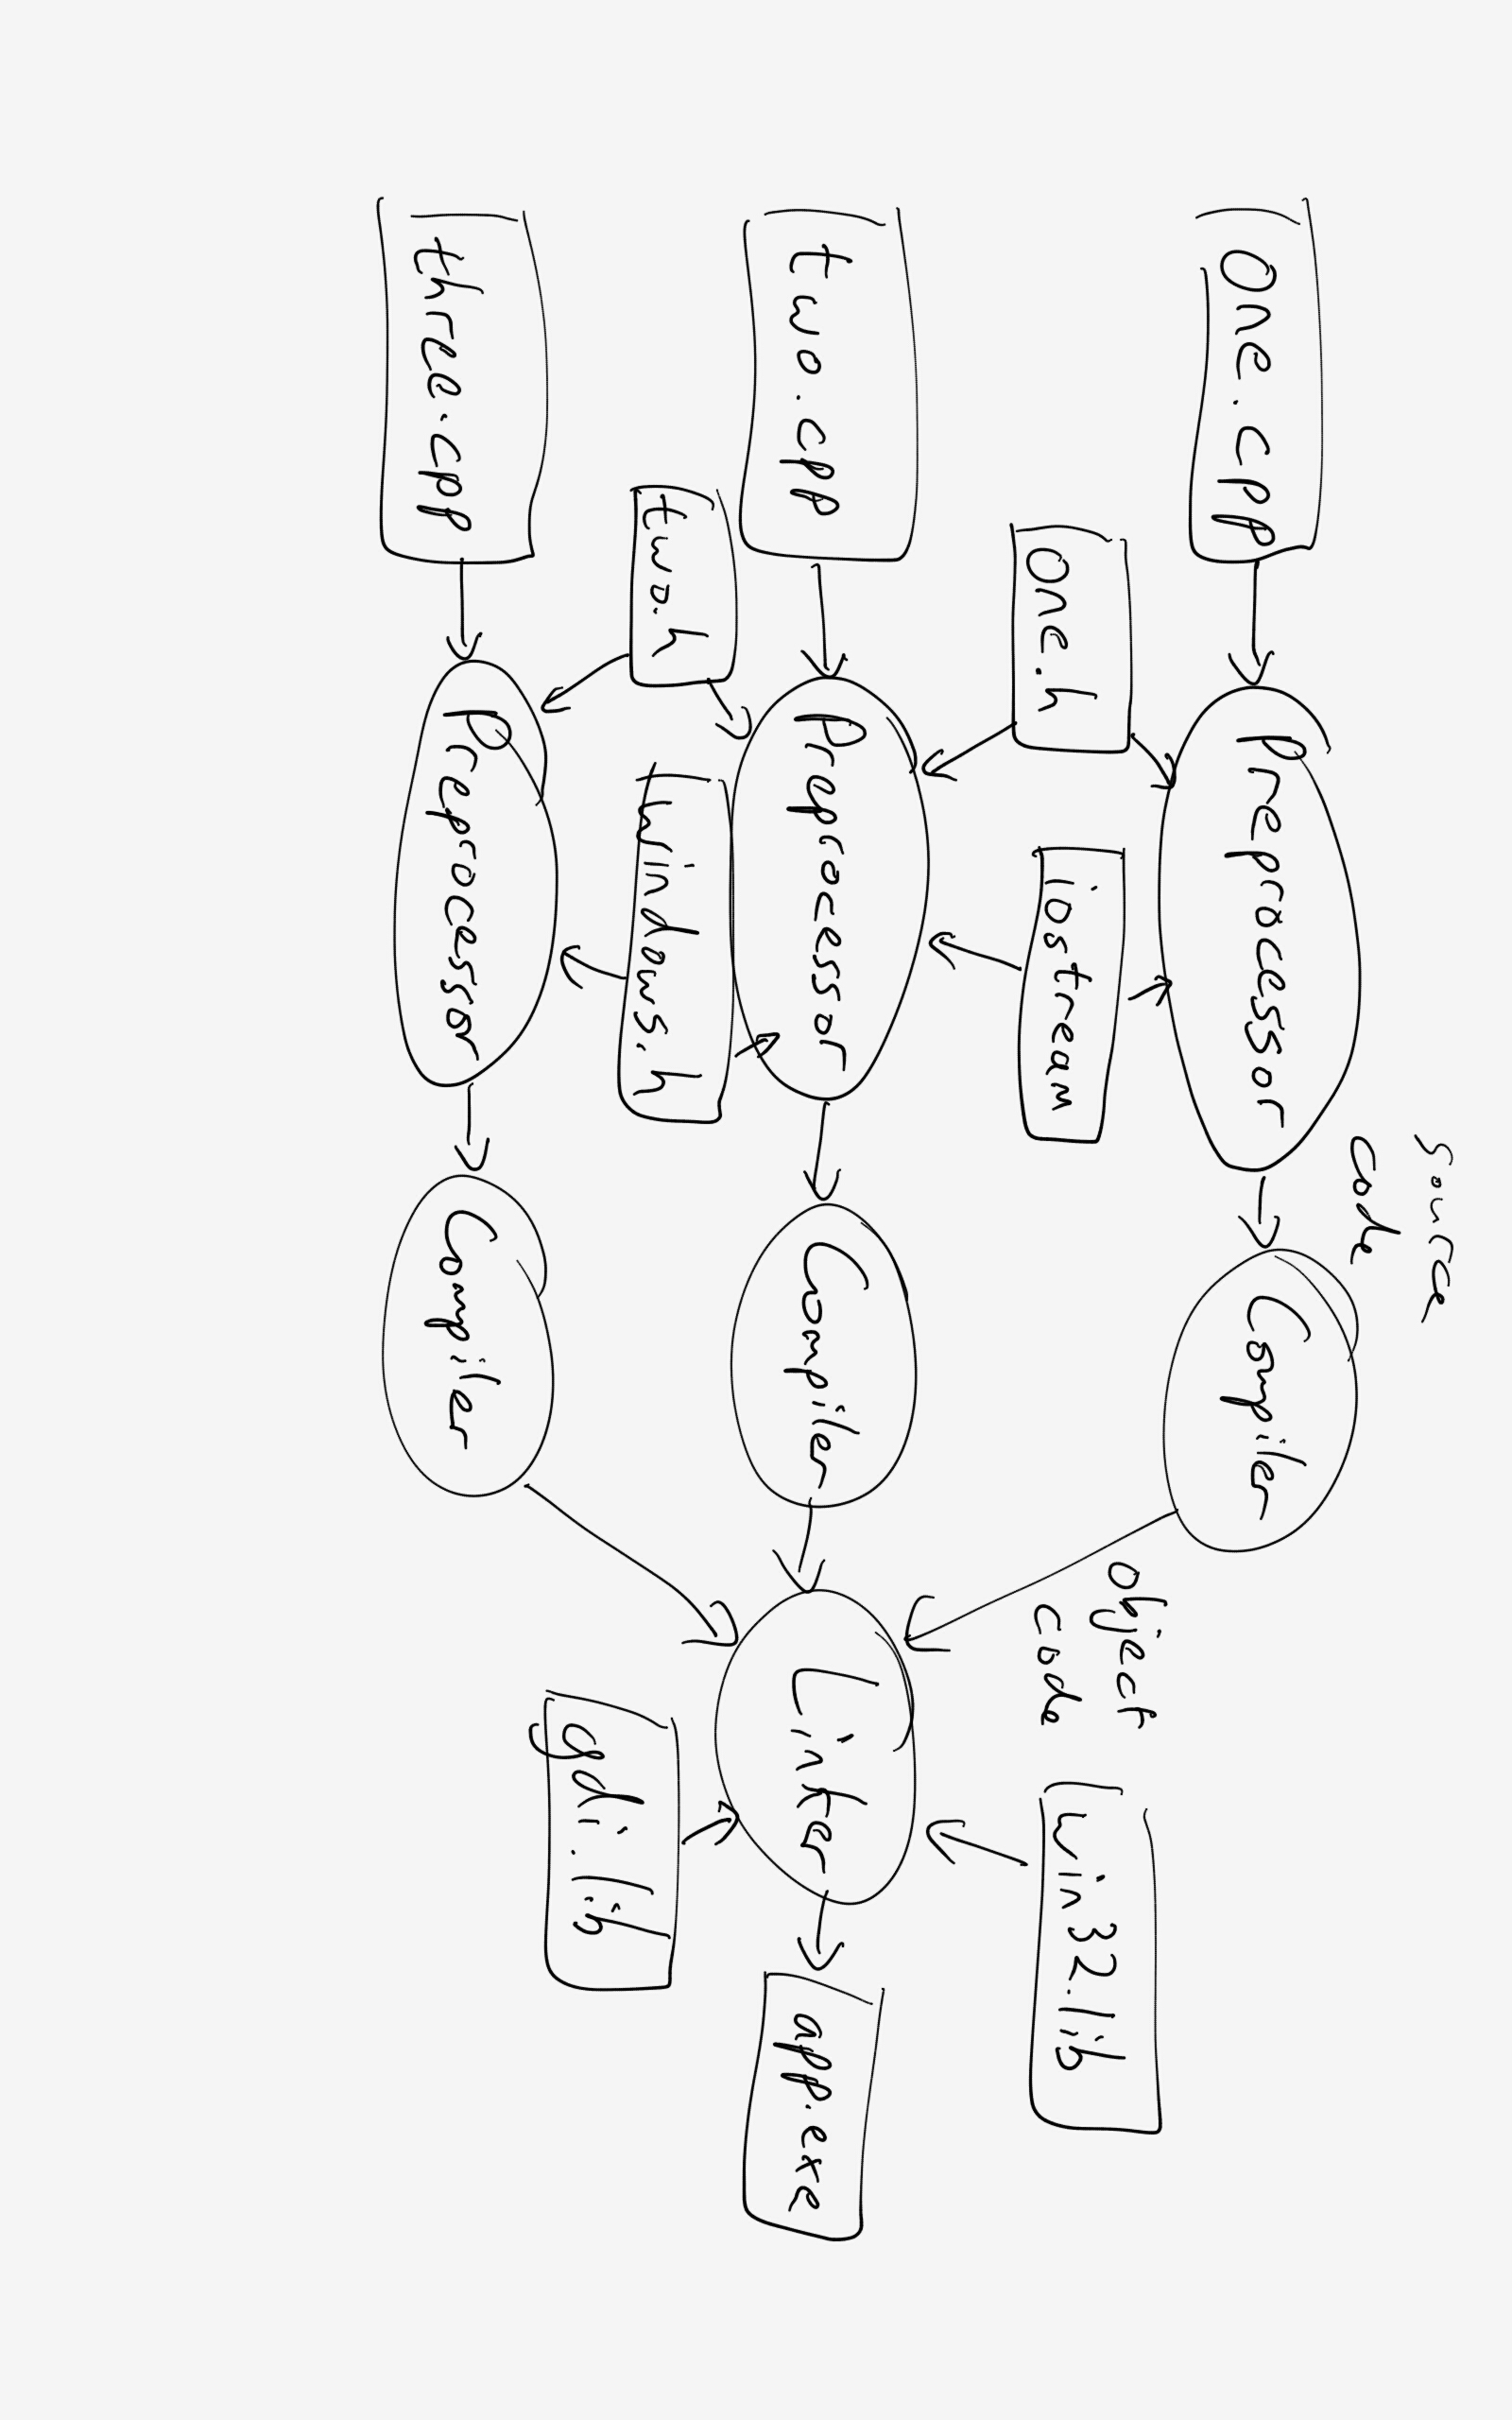
\includegraphics[height=\textwidth,angle=90]{compiler_sketch}
%\end{frame}

\end{document}
